% ---------------------------------------------------------------------------- %
% ---------------------- Starter Guide - Italian Version --------------------- %
% ---------------------------------------------------------------------------- %
%
%
% This document is meant as a starter guide for people approaching MATLAB and
% the Data science courses for economy students for the first time. It is
% intended to offer guidance on the first step while approaching the subject. 
% ---------------------------------------------------------------------------- %
% Covered topics: - MATLAB installation 
% --------------------------------- Preamble --------------------------------- %
\documentclass[a4paper, 12pt]{article}
\usepackage{graphicx}
\usepackage[italian]{babel}
\usepackage{url}
\usepackage{microtype}
\usepackage[indent=0pt]{parskip} %par skips a line and remove paragraphs indent
\usepackage{hyperref}
\hypersetup{colorlinks=true, 
            linkcolor=blue, 
            citecolor=blue, 
            urlcolor=blue
            }
\usepackage{caption}
\usepackage{subcaption}
\captionsetup[figure]{labelformat=empty}
% \captionsetup[subfigure]{labelformat=empty} % unused
\usepackage[autostyle,italian=quotes]{csquotes}
\usepackage{listings}

\lstset{basicstyle=\normalsize\ttfamily,breaklines=false}
%------------------------------------------------------------------------------
% title information
\title{Data Science con MATLAB\\
\large{Guida Introduttiva}}
\date{}
\author{}
% table of contents
\addto\captionsitalian{\renewcommand{\contentsname}{Indice della guida:}}
% directory of the images
\graphicspath{{Images/}}
%--------------------------------------------------------------------------------
\begin{document}
\maketitle % Title
% little introductio paragraph
\begin{center}
\begin{minipage}{0.95\textwidth}
\textbf{Serve aiuto?} \hfill \break
Se ti capita di incontrare difficoltà con l'installazione o con l'utilizzo di
MATLAB materiale di corredo, ricordati sempre che puoi ricevere aiuto dal
professore, o da altri studenti sulla pagina GitHub del libro riportata nella
sezione \hyperref[sec:GitHub]{\enquote{4.1 GitHub}} di questa guida.\hfill
\end{minipage}
\end{center}

%Table of Contents
\tableofcontents

% Start of the guide
\newpage

% Sections regarding the license part has been removed from the italian version
% since it is assumed that students at the second and third year of the
% economics course will surely already have their UNIPR email. If it is deemed
% necessary, they can always be added in a later version.

\section{Installare MATLAB}\label{sec:MATinstall} Per installare MATLAB è
necessario avere una licenza in corso di validità; utilizzando la tua email
universitaria, avrai accesso gratuitamente ad una licenza MATLAB fornita
dall'Università di Parma.

\subsection{Installazione del programma}
Per installare MATLAB, segui questi passi:

\begin{enumerate}
	\item Dirigiti al seguente link:
	      \href{https://www.mathworks.com/downloads/}{mathworks.com/downloads},
	      seleziona la versione che vuoi scaricare (solitamente l'ultima uscita,
	      a meno che tu non abbia esigenze particolari). Un programma per
	      l'installazione guidata verrà scaricato sul tuo PC.
	      	      
	\item Ora, trova il programma che hai appena scaricato sul tuo PC
	    (solitamente nella cartella \textbf{Downloads}), fai doppio clic su di
	    esso ed eseguilo. In questo modo inizierà la procedura guidata per
	    l'installazione.
	      	      
	\item Ti verrà chiesto di selezionare una licenza: selezionala e procedi.
	      	      
	\item Scegli una cartella per l'installazione. Se non hai preferenze, lascia
	pure quella predefinita.
	      	      
	\item Seleziona quali prodotti vuoi installare. Per questo corso sono
	necessari i seguenti Toolbox:
	      \begin{itemize}
	      	\item MATLAB
	      	\item Datafeed Toolbox
	      	\item Econometrics Toolbox
	      	\item Financial Toolbox
	      	\item Image Processing Toolbox
	      	\item Mapping Toolbox
		    \item Optimization Toolbox		
	      	\item Parallel Computing Toolbox
	      	\item Risk Management Toolbox
	      	\item Statistics and Machine Learning Toolbox
	      \end{itemize}
	    
	\item Seleziona ulteriori opzioni a seconda delle tue preferenze e inizia il
	processo di installazione. Una barra di avanzamento mostrerà l'andamento del
	processo e, al completamento dell'operazione, apparirà un messaggio sullo
	schermo. Dopo aver completato l'installazione di MATLAB, procedi alla
	prossima sezione per installare il Toolbox FSDA.
\end{enumerate}

\subsection{Installazione di FSDA}
Ci siamo quasi! Ora devi solo installare il toolbox FSDA dall'Add-On Explorer di
MATLAB.\par

FSDA, ovvero Flexible Statistics and Data Analysis Toolbox, estende le
funzionalità di MATLAB e dello Statistics and Machine Learning Toolbox per
supportare un'analisi robusta ed efficiente di dataset complessi influenzati da
diverse fonti di eterogeneità.\par

\begin{enumerate}
	\item Apri MATLAB e guarda nella barra degli strumenti in alto. Assicurati
	di essere nella sezione \enquote{HOME}, trova il pulsante \textbf{Add-Ons} e
	cliccaci sopra.

	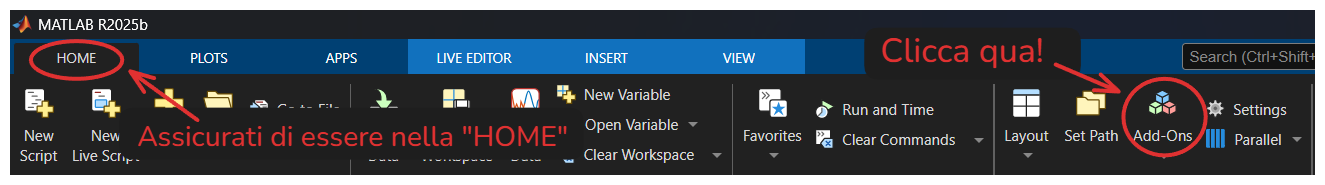
\includegraphics[width=.9\textwidth]{Matlab_header.png}

	\item L'Add-On Explorer di MATLAB si aprirà. Apri la barra di ricerca, scrivi
	\textbf{FSDA} e premi invio. Il primo risultato dovrebbe essere quello
	corretto: cliccalo.

	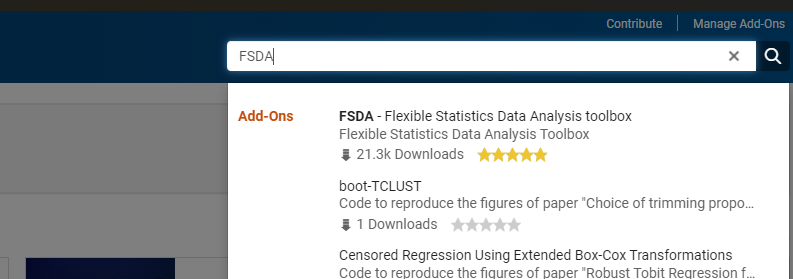
\includegraphics[width=.9\textwidth]{FSDA.png}

	\item Clicca su \textbf{Add}: il processo di download e installazione del
	toolbox inizierà. Attendi che il processo sia finito.

	\item FSDA è un progetto vivo e viene aggiornato spesso, per cui ogni tanto
	ricordati di utilizzare la funzione \texttt{\textbf{tuna}} per assicurarti
	di avere sempre l'ultima versione di FSDA.\hfill \break
	Per utilizzare questa funzione, scrivi \texttt{\textbf{tuna}} nella command
	window di MATLAB, se la tua versione di FSDA è obsoleta, ti verrà
	consigliato di aggiornare il toolbox attraverso l'Add-On Manager.
\end{enumerate}

\section{Domande Frequenti}
\subsection{Licenza non utilizzabile}
Se durante l'installazione o l'accesso al sito web di MathWorks, vi capita di visualizzare il seguente messaggio:

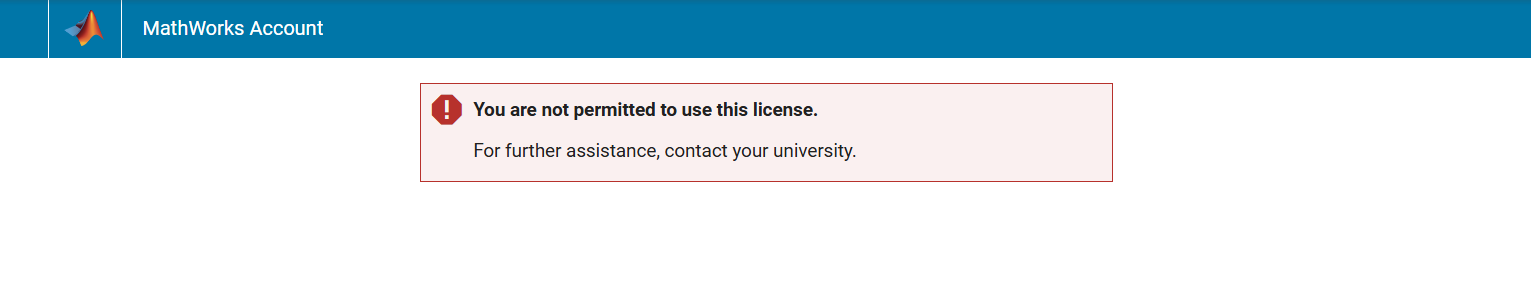
\includegraphics[width=.9\textwidth]{MATLAB-LICENSE-ISSUE-cropped.png}

La soluzione è spesso quella di inviare una email al seguente indirizzo: \href{mailto:helpdesk.informatico@unipr.it}{helpdesk.informatico@unipr.it}, contenente il vostro nome, cognome, corso e email universitaria, in cui descrivete dettagliatamente il messaggio di errore che vedete.
\end{document}